\chapter{Topic-wise gossip scheduling model}\label{sec:appendix_gossip_model}

This appendix is the analytical model that backs the sharded gossip design
sketched in section~\ref{sec:session_gossip}. It estimates the mean gossip
arrival rate observed at a node as a function of the total topic count, the
number of topics the node joins, and the mean sharing multiplicity of those
topics. It is non-normative and is reproduced from the
\texttt{model/gossip\_propagation.ipynb} notebook of the Cy reference
implementation.

The session layer defines the gossip rate on a \emph{per-topic} basis. Each
topic induces its own network-wide gossip process with mean rate $r_t$, and
the deduplication rules in section~\ref{sec:session_gossip_suppression} keep
this rate approximately invariant with respect to the number of nodes sharing
the topic. As a consequence, the mean inter-gossip interval for any particular
topic is $1/r_t$ regardless of how many nodes hold that topic, which is an
essential trait that allows resource-constrained nodes to participate in large networks.

The trade-off is that the \emph{per-node} gossip rate now scales linearly
with the number of topics the node holds, so the per-topic rate $r_t$ must be
kept low.

\begin{remark}
    For better consensus observability, the first gossip of a newly created
    local topic is always broadcast, and implementations may elect to
    tentatively raise the gossip rate for topics that are new, have recently
    seen collisions or divergences, or are joined by a single node. These
    refinements do not affect the model below and can be factored in
    trivially.
\end{remark}

\section{Notation}

Let:

\begin{description}
    \item[$K$] the set of all non-pinned topics present on the network, with
    $|K| = K_{\text{total}}$.
    \item[$S_x \subseteq K$] the set of topics used by node $x$, with
    $K_x = |S_x|$.
    \item[$M_t$] the set of nodes using topic $t$, with $m_t = |M_t|$.
    \item[$g(t)$] the gossip shard assigned to topic $t$, taken from
    $\{1, 2, \ldots, G\}$ where $G$ is the number of gossip shards
    (section~\ref{sec:session_subject_id_mapping}).
    \item[$T_x$] the set of shards joined by node $x$, i.e.
    $T_x = \{g(t) : t \in S_x\}$, with $U_x = |T_x|$.
    \item[$r_t$] the mean network-wide gossip rate of topic $t$ after
    deduplication.
    \item[$b_t$] the fraction of gossip messages for topic $t$ that are sent
    on the broadcast subject instead of the topic's shard.
    \item[$\pi_{x,t}$] the probability that node $x$ is the emitter when
    topic $t$ is gossiped.
\end{description}

\section{Derivation}

Under these definitions, the mean arrival rate at node $x$ is
\begin{equation*}
    R_x = \sum_{t \in K} r_t\,(1 - \pi_{x,t})
          \left[ b_t + (1 - b_t)\,\mathbf{1}\{g(t) \in T_x\} \right]
\end{equation*}
where $\mathbf{1}\{\cdot\}$ is the indicator function. The first factor
accounts for the fact that node $x$ does not receive gossip it emits itself;
the bracketed term splits the remaining traffic between broadcast gossip
(received regardless of shard membership) and sharded gossip (received only
if node $x$ joins the shard).

Assuming that the deduplication rules distribute transmission opportunities
fairly among the nodes sharing a topic,
\begin{equation*}
    \pi_{x,t} \approx
    \begin{cases}
        \frac{1}{m_t}, & x \in M_t \\
        0,             & x \notin M_t
    \end{cases}
\end{equation*}
Splitting the sum by whether the topic is used by node $x$ gives
\begin{equation*}
    R_x \approx
    \sum_{t \in S_x} r_t \left(1 - \frac{1}{m_t}\right)
    + \sum_{t \notin S_x} r_t
      \left[ b_t + (1 - b_t)\,\mathbf{1}\{g(t) \in T_x\} \right]
\end{equation*}
For topics that $x$ holds, the broadcast fraction $b_t$ does not appear
because node $x$ receives every remote gossip of its own topics anyway, on
whichever carrier.

Assume random shard assignment and no correlation between unrelated topics;
then for a topic $t \notin S_x$,
\begin{equation*}
    \mathbb{P}\bigl(g(t) \in T_x\bigr) \approx \frac{U_x}{G}
\end{equation*}
which yields
\begin{equation*}
    \mathbb{E}[R_x] \approx
    \sum_{t \in S_x} r_t \left(1 - \frac{1}{m_t}\right)
    + \sum_{t \notin S_x} r_t
      \left[ b_t + (1 - b_t)\,\frac{U_x}{G} \right]
\end{equation*}

Specializing to a homogeneous network with $r_t = r$ and $b_t = b$:
\begin{equation*}
    \mathbb{E}[R_x] \approx
    r \sum_{t \in S_x}\left(1 - \frac{1}{m_t}\right)
    + r\,(K_{\text{total}} - K_x)
      \left[ b + (1 - b)\,\frac{U_x}{G} \right]
\end{equation*}
If the topics $x$ holds have approximately the same mean sharing multiplicity
$\bar m_x$, this simplifies to
\begin{equation*}
    \mathbb{E}[R_x] \approx
    r\,K_x\left(1 - \frac{1}{\bar m_x}\right)
    + r\,(K_{\text{total}} - K_x)
      \left[ b + (1 - b)\,\frac{U_x}{G} \right]
\end{equation*}
A higher $\bar m_x$ means node $x$ is more likely to hear its topics
gossiped by somebody else and suppress its own emissions accordingly; the
limit $\bar m_x = 1$ (only node $x$ holds the topic) removes the first term
entirely because no one else generates arrival load for those topics.

If local shard collisions are rare, $U_x \approx K_x$ and the expression
reduces further to
\begin{equation*}
    \mathbb{E}[R_x] \approx
    r\,K_x\left(1 - \frac{1}{\bar m_x}\right)
    + r\,(K_{\text{total}} - K_x)
      \left[ b + (1 - b)\,\frac{K_x}{G} \right]
\end{equation*}
This final form is not directly dependent on the node count $N$; instead it
depends on the total topic count, the number of topics the local node joins,
and the mean sharing multiplicity of the node's own topics.

\section{Numerical example}

Figure~\ref{fig:appendix_gossip_model_topicwise} plots the arrival load at a
node as a function of the total topic count $K_{\text{total}}$ and the
number of joined topics $K_x$, with $b = 0.1$, $r = 0.2$~Hz, $G = 1984$, and
the limit case $\bar m_x \to \infty$ (the worst case for receive-only load,
where the local node never gets to suppress an emission of its own).

\begin{figure}[H]
    \centering
    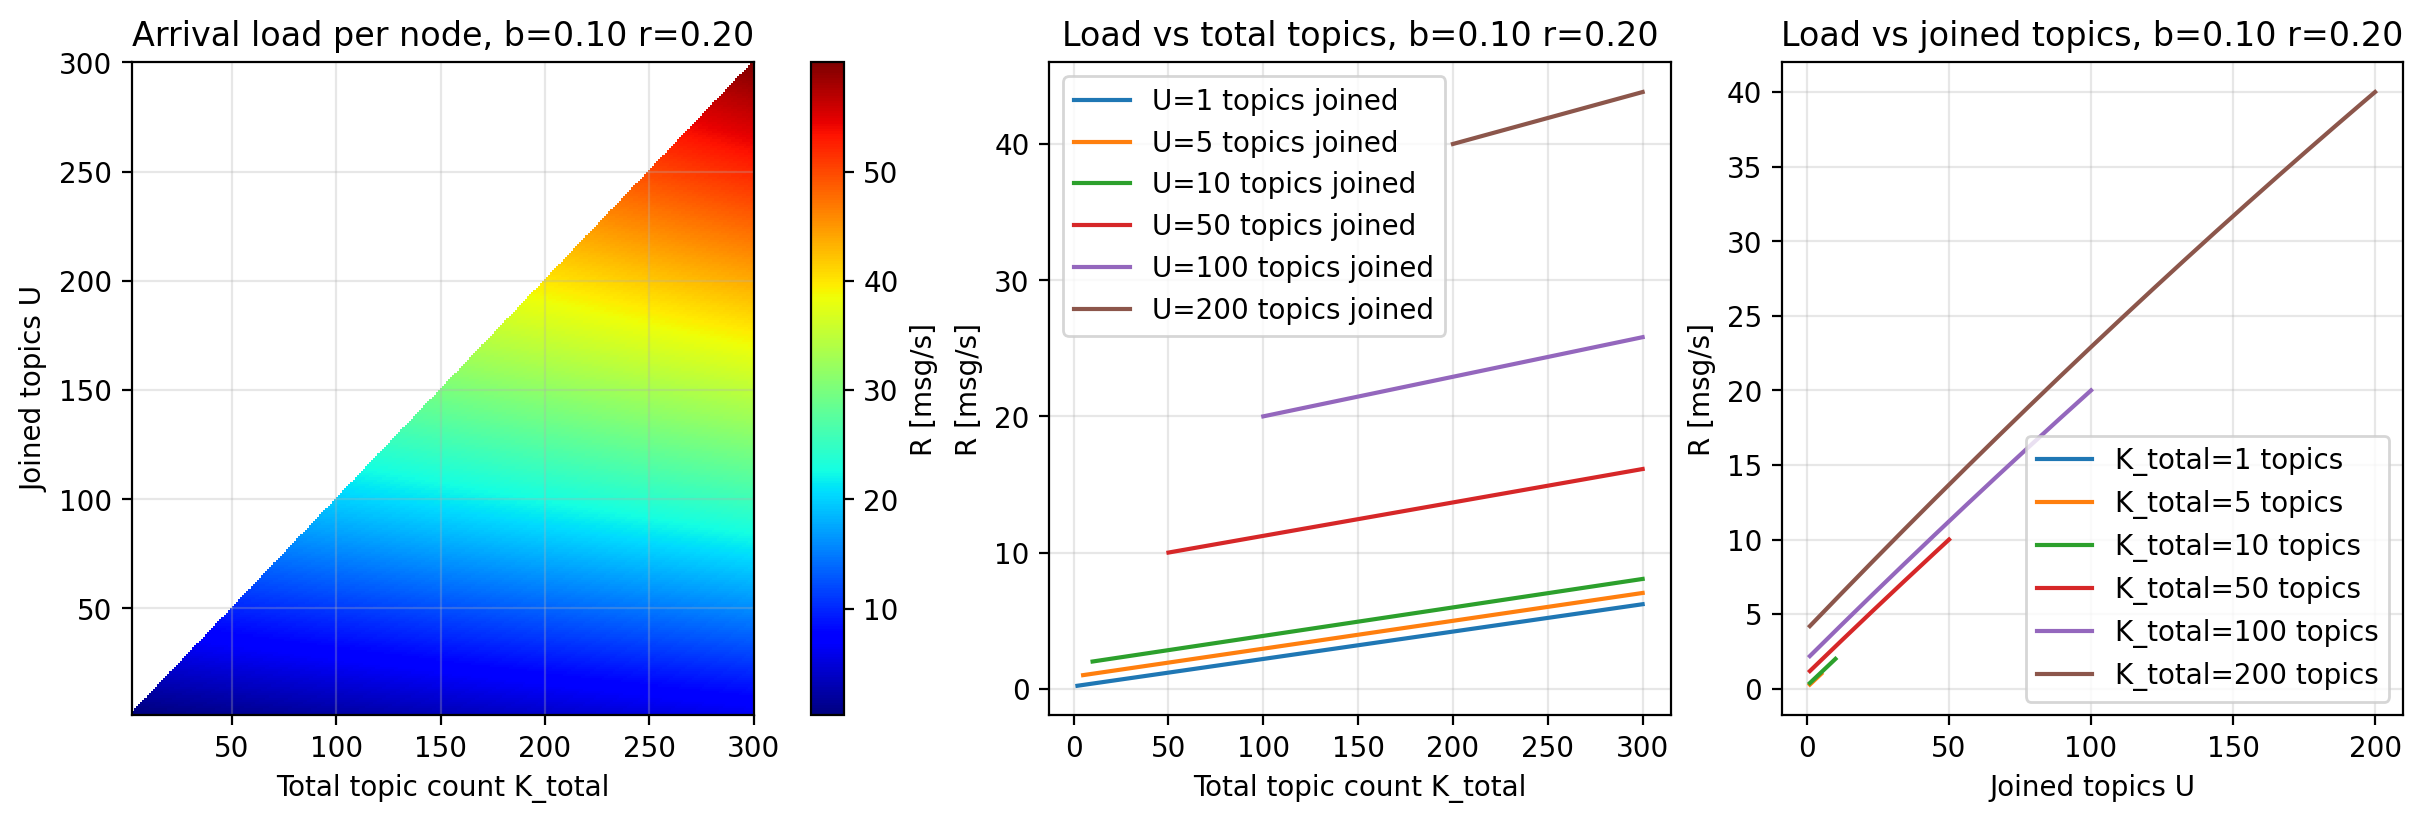
\includegraphics[width=\textwidth]{appendices/topicwise_gossip_load.png}
    \caption{Topic-wise gossip arrival load model}
    \label{fig:appendix_gossip_model_topicwise}
\end{figure}

The heat map on the left shows the arrival rate as a function of the two
parameters; the middle and right panels slice it along constant $K_x$ and
constant $K_{\text{total}}$ respectively.
The key observation is that this design is compatible with resource-limited nodes because the network participation
load scales primarily with the number of topics that the node joins,
which is a parameter it controls and that is also small in resource-limited nodes,
as opposed to the total number of participants in the network.
This enables resource-limited nodes to participate in large networks.
